% -*- latex -*-
%%%%%%%%%%%%%%%%%%%%%%%%%%%%%%%%%%%%%%%%%%%%%%%%%%%%%%%%%%%%%%%%
%%%%%%%%%%%%%%%%%%%%%%%%%%%%%%%%%%%%%%%%%%%%%%%%%%%%%%%%%%%%%%%%
%%%%
%%%% This text file is part of the lecture slides for
%%%% `Parallel Computing'
%%%% by Victor Eijkhout, copyright 2012-2022
%%%%
%%%% Atomic-slides.tex : slides about atomic one-sided communication
%%%%
%%%%%%%%%%%%%%%%%%%%%%%%%%%%%%%%%%%%%%%%%%%%%%%%%%%%%%%%%%%%%%%%
%%%%%%%%%%%%%%%%%%%%%%%%%%%%%%%%%%%%%%%%%%%%%%%%%%%%%%%%%%%%%%%%

\begin{numberedframe}{Justification}
  MPI-1/2 lacked tools for race condition-free one-sided communication.\\
  These have been added in MPI-3.
\end{numberedframe}

\begin{numberedframe}{Emulating shared memory with one-sided communication}
  \begin{itemize}
  \item One process stores a table of work descriptors, and a `stack pointer'
    stating how many there are.
  \item Each process reads the pointer, reads the corresponding
    descriptor, and decrements the pointer; and
  \item A process that has read a descriptor then executes the
    corresponding task.
  \item Non-collective behavior: processes only take a descriptor when they are available.
  \end{itemize}
\end{numberedframe}

\begin{numberedframe}{In a picture}
  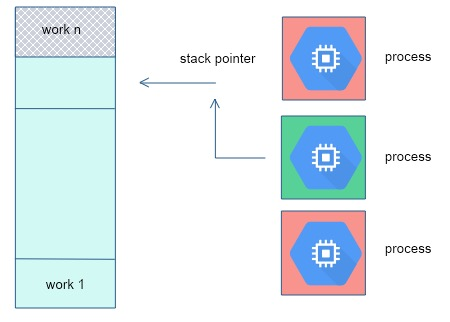
\includegraphics[scale=.5]{workpool}
\end{numberedframe}

\begin{numberedframe}{Simplified model}
  \begin{itemize}
  \item One process has a counter, which models the shared memory;
  \item Each process, if available, reads the counter; and
  \item \ldots~decrements the counter.
  \item No actual work: random decision if process is available.
  \end{itemize}
\end{numberedframe}

\begin{numberedframe}{Shared memory problems: what is a race condition?}
  \scriptsize
  Race condition: outward behavior depends on
  timing/synchronization of low-level events.\\
  In shared memory associated with shared data.

  Example:
  \begin{tabbing}
    Init: \texttt{I=0}\\
    process 1: \texttt{I=I+2}\\
    process 2: \texttt{I=I+3}
  \end{tabbing}
  \begin{tabular}{|rr|rr|rr|}
    \hline
    \multicolumn{2}{|c|}{scenario 1.}& \multicolumn{2}{|c|}{scenario 2.}&
    \multicolumn{2}{|c|}{scenario 3.}\\ \hline
    \multicolumn{6}{|c|}{$\n{I}=0$}\\ \hline
    read $\n{I}=0$&read $\n{I}=0$&
    read $\n{I}=0$&read $\n{I}=0$&
    read $\n{I}=0$& \\
    local $\n{I}=2$&local $\n{I}=3$& 
    local $\n{I}=2$&local $\n{I}=3$&
    local $\n{I}=2$& \\
    write $\n{I}=2$& & &write $\n{I}=3$&write $\n{I}=2$& \\
    &write $\n{I}=3$&write $\n{I}=2$& & &read $\n{I}=2$\\
    &&&&&local $\n{I}=5$\\
    &&&&&write $\n{I}=5$\\
    \hline
    \multicolumn{2}{|c|}{$\n{I}=3$}& \multicolumn{2}{|c|}{$\n{I}=2$}&
    \multicolumn{2}{|c|}{$\n{I}=5$}\\ \hline
  \end{tabular}

  (In MPI, the read/write would be \indexmpishow{MPI_Get}~/ \indexmpishow{MPI_Put} calls)
\end{numberedframe}

\begin{numberedframe}{Case study in shared memory: 1, wrong}
  \label{sl:fetchput}
  \cverbatimsnippet{countdowngetput}
\end{numberedframe}

\begin{numberedframe}{Discussion}
  \begin{itemize}
  \item The multiple \indexmpishow{MPI_Put} calls conflict.
  \item Code is correct if in each iteration there is only one writer.
  \item Question: In that case, can we take out the middle fence?
  \item Question: what is wrong with
\begin{lstlisting}
MPI_Win_fence(0,the_window);
if (i_am_available) {
  MPI_Get( &counter_value, ... )
  MPI_Win_fence(0,the_window);
  MPI_Put( ... )      
}
MPI_Win_fence(0,the_window);
\end{lstlisting}
?
  \end{itemize}
\end{numberedframe}

\begin{numberedframe}{Case study in shared memory: 2, hm}
  \label{sl:fetchacc}
  \cverbatimsnippet{countdowngetacc}
\end{numberedframe}

\begin{numberedframe}{Discussion: need for atomics}
  \label{sl:fetchop}
  \begin{itemize}
  \item \indexmpishow{MPI_Accumulate} is atomic, so no conflicting writes.
  \item What is the problem?
  \item Answer: Processes are not reading unique \lstinline+counter_value+ values.
  \item Conclusion: Read and update need to come together:\\
    read unique value and immediately update.
  \end{itemize}
  Atomic `get-and-set-with-no-one-coming-in-between':\\
  \indexmpishow{MPI_Fetch_and_op}~/ \indexmpishow{MPI_Get_accumulate}.\\
  Former is simple version: scalar only.
\end{numberedframe}

\protoslide{MPI_Fetch_and_op}

\begin{numberedframe}{Case study in shared memory: 3, good}
  \label{sl:fetchaccgood}
  \cverbatimsnippet{fetchopfence}
\end{numberedframe}

\begin{numberedframe}{Allowable operators. (Hint!)}
  \input mpi-opstable

  No user-defined operators.
\end{numberedframe}

\begin{numberedframe}{Problem}
  We are using fences, which are collective.\\
  What if a process is still operating on its local work?

  Better (but more tricky) solution:\\
  use passive target synchronization and locks.
\end{numberedframe}

\begin{numberedframe}{Passive target epoch}
\begin{lstlisting}
if (rank == 0) {
  MPI_Win_lock (MPI_LOCK_EXCLUSIVE, 1, 0, win);
  MPI_Put (outbuf, n, MPI_INT, 1, 0, n, MPI_INT, win);
  MPI_Win_unlock (1, win);
}
\end{lstlisting}
No action on the target required!  
\end{numberedframe}

\begin{exerciseframe}[lockfetch]
  \input ex:lockandfetch
\end{exerciseframe}

\begin{solutions}
\begin{solution}
  Update shared window:
  \cverbatimsnippet{workerop}
  Read-out of counter value:
  \cverbatimsnippet{managerread}
\end{solution}
\end{solutions}

\begin{exerciseframe}[lockfetchshared]
  \input ex:lockfetchshared
\end{exerciseframe}

\begin{solutions}
\begin{solution}
  \begin{multicols}{2}
    \cverbatimsnippet{sharedlockupdate}
  \end{multicols}
\end{solution}
\end{solutions}

\endinput

\begin{numberedframe}{}
  \label{sl:}
\end{numberedframe}

%% this is already covered by the previous slides, not?
\begin{optexerciseframe}
  \input ex:countdownop
\end{optexerciseframe}

